\documentclass[a4paper]{article}

\usepackage{inputenc}
\usepackage[british,UKenglish]{babel}
\usepackage{amsmath}
%\usepackage{titlesec}
\usepackage{color}
\usepackage{graphicx}
\usepackage{fancyref}
\usepackage{hyperref}
\usepackage{float}
\usepackage{scrextend}
\usepackage{setspace}
\usepackage{xargs}
\usepackage{multicol}
\usepackage{nameref}

\usepackage{sectsty}
\usepackage{multicol}
\usepackage{multirow}
\usepackage[procnames]{listings}
\usepackage{appendix}

\newcommand\tab[1][1cm]{\hspace*{#1}}
\hypersetup{colorlinks=true, linkcolor=black}
\interfootnotelinepenalty=10000

\newcommand{\cleancode}[1]{\begin{addmargin}[3em]{3em}\texttt{\textcolor{cleanOrange}{#1}}\end{addmargin}}
\newcommand{\cleanstyle}[1]{\text{\textcolor{cleanOrange}{\texttt{#1}}}}


\usepackage[colorinlistoftodos,prependcaption,textsize=footnotesize]{todonotes}
\newcommandx{\commred}[2][1=]{\textcolor{Red}
{\todo[linecolor=red,backgroundcolor=red!25,bordercolor=red,#1]{#2}}}
\newcommandx{\commblue}[2][1=]{\textcolor{Blue}
{\todo[linecolor=blue,backgroundcolor=blue!25,bordercolor=blue,#1]{#2}}}
\newcommandx{\commgreen}[2][1=]{\textcolor{OliveGreen}{\todo[linecolor=OliveGreen,backgroundcolor=OliveGreen!25,bordercolor=OliveGreen,#1]{#2}}}
\newcommandx{\commpurp}[2][1=]{\textcolor{Plum}{\todo[linecolor=Plum,backgroundcolor=Plum!25,bordercolor=Plum,#1]{#2}}}

\def\code#1{{\tt #1}}

\def\note#1{\noindent{\bf [Note: #1]}}

\makeatletter
%% The "\@seccntformat" command is an auxiliary command
%% (see pp. 26f. of 'The LaTeX Companion,' 2nd. ed.)
\def\@seccntformat#1{\@ifundefined{#1@cntformat}%
   {\csname the#1\endcsname\quad}  % default
   {\csname #1@cntformat\endcsname}% enable individual control
}
\let\oldappendix\appendix %% save current definition of \appendix
\renewcommand\appendix{%
    \oldappendix
    \newcommand{\section@cntformat}{\appendixname~\thesection\quad}
}
\makeatother


% "define" Scala
\usepackage[T1]{fontenc}  
\usepackage[scaled=0.82]{beramono}  
\usepackage{microtype} 

\sbox0{\small\ttfamily A}
\edef\mybasewidth{\the\wd0 }

\lstdefinelanguage{scala}{
  morekeywords={abstract,case,catch,class,def,%
    do,else,extends,false,final,finally,%
    for,if,implicit,import,match,mixin,%
    new,null,object,override,package,%
    private,protected,requires,return,sealed,%
    super,this,throw,trait,true,try,%
    type,val,var,while,with,yield},
  sensitive=true,
  morecomment=[l]{//},
  morecomment=[n]{/*}{*/},
  morestring=[b]",
  morestring=[b]',
  morestring=[b]"""
}

\usepackage{color}
\definecolor{dkgreen}{rgb}{0,0.6,0}
\definecolor{gray}{rgb}{0.5,0.5,0.5}
\definecolor{mauve}{rgb}{0.58,0,0.82}

% Default settings for code listings
\lstset{frame=tb,
  language=scala,
  aboveskip=3mm,
  belowskip=3mm,
  showstringspaces=false,
  columns=fixed, % basewidth=\mybasewidth,
  basicstyle={\small\ttfamily},
  numbers=none,
  numberstyle=\footnotesize\color{gray},
  % identifierstyle=\color{red},
  keywordstyle=\color{blue},
  commentstyle=\color{dkgreen},
  stringstyle=\color{mauve},
  frame=single,
  breaklines=true,
  breakatwhitespace=true,
  procnamekeys={def, val, var, class, trait, object, extends},
  procnamestyle=\ttfamily\color{red},
  tabsize=2
}

\lstnewenvironment{scala}[1][]
{\lstset{language=scala,#1}}
{}
\lstnewenvironment{cpp}[1][]
{\lstset{language=C++,#1}}
{}
\lstnewenvironment{bash}[1][]
{\lstset{language=bash,#1}}
{}
\lstnewenvironment{verilog}[1][]
{\lstset{language=verilog,#1}}
{}



\lstset{frame=,basicstyle={\footnotesize\ttfamily}}



\graphicspath{ {images/} }
\usepackage{ctex}
\usepackage{verbatim}
\usepackage{enumerate}
\usepackage{geometry}
\usepackage{amssymb}
\usepackage{amsmath}
%\usepackage{slashbox}
\usepackage{diagbox}
\usepackage{pifont}%\ding{192} \ding{172}
\usepackage{tikz}
\usepackage{booktabs}
%\geometry{a4paper, scale=0.72}
\geometry{a4paper,left=2.5cm,right=2.5cm,top=2.5cm,bottom=2.5cm}
%%%%%%%%%%%%%%%%%%%%%%%%%%%%%%%%%%%%%%%% BEGIN DOC %%%%%%%%%%%%%%%%%%%%%%%%%%%%%%%%%%%%%%%%

\begin{document}
\setlength{\abovecaptionskip}{0pt}
\setlength{\belowcaptionskip}{0pt}
\renewcommand{\contentsname}{目\ 录}
\renewcommand{\appendixname}{附录}
\renewcommand{\appendixpagename}{附录}
\renewcommand{\refname}{参考文献} 
\renewcommand{\figurename}{图}
\renewcommand{\tablename}{表}
\renewcommand{\today}{\number\year 年 \number\month 月 \number\day 日}
\renewcommand{\comma}{$\mkern -8.5mu\raise -.2ex\hbox{\rotatebox[]{180}{\`}}\ $}

\newcommand*{\circled}[1]{\lower.7ex\hbox{\tikz\draw (0pt, 0pt)%
    circle (.5em) node {\makebox[1em][c]{\small #1}};}}
\title{{\Huge 近代物理实验报告{\large\linebreak\\}}{\Large 实验2-2:\ 符合测量\linebreak\linebreak}}
%please write your name, Student #, and Class # in Authors, student ID, and class # respectively
\author{\\姓\ 名:付\ 大\ 为\\
学\ 号: 1800011105\\
邮\ 箱: \url{fudw@pku.edu.cn}\\
%班\ 号: xxxxx\\\\
近代物理实验 (I)\\
(2021,秋季学期)\\\\
北京大学\\
物理学院\\
2018级1班}
\date{\today}
\maketitle
\newpage

%%%%%%%%%%%%%%%%%%%%%%%%%%%%%%%%%%%%%%%% ABSTRACT %%%%%%%%%%%%%%%%%%%%%%%%%%%%%%%%%%%%%%%%
\begin{center}
{\Large\bf{摘\ 要\\}}
\end{center}

符合测量技术是核物理实验的主要的、基本的实验技术之一,在各领域有着广泛应用,在核反应的研究中,可以用来确定反应物的能量和角分布;在核衰变测量中可以用来研究核衰变机制、级联辐射之间的角关联、短寿命放射性核素的半衰期等.符合事件是指两个或两个以上同时发生的事件,具有内在因果关系的符合输出称为真符合,不具有相关性的事件间的符合称为偶然符合.不同时发生的相关事件,可以把其中一个事件的脉冲延迟与另一个事件脉冲同时到达符合电路而产生符合脉冲,这种符合称之为延迟符合.$\beta$探测器用塑料闪烁体来测量$\beta$粒子;$\gamma$探测器用NaI(Tl)闪烁体,另外有铝屏蔽罩,将$\mathrm \sideset{^{60}}{}Co$发出的$\beta$射线完全挡住,因而只能测量$\gamma$射线.本实验的目的是学习符合测量的基本方法、测量符合装置的分辨时间和用$\beta-\gamma$符合测$\mathrm \sideset{^{60}}{}Co$的放射性活度.\\\\
{\bf{关键词}:}符合测量, 延迟符合, 放射性活度
\newpage

%%%%%%%%%%%%%%%%%%%%%%%%%%%%%%%%%%%%%%%% CONTENT %%%%%%%%%%%%%%%%%%%%%%%%%%%%%%%%%%%%%%%%
\begin{center}
\tableofcontents\label{c}
\end{center}
\newpage

%%%%%%%%%%%%%%%%%%%%%%%%%%%%%%%%%%%%%%%% Introduction %%%%%%%%%%%%%%%%%%%%%%%%%%%%%%%%%%%%%%%%
\section{引言} \label{overview}%------------------------------
用闪烁计数器或盖革-米勒计数器对放射源活度作绝对测量时比较困难的.这是因为绝对测量需要对影响测量结果(计数率)的许多因素,如立体角、计数效率、计数器分辨时间、散射和吸收、源的自吸收等进行修正,而上述因素一般都很难准确测定,对于衰变时有级联辐射的放射性元素,用符合法来测量则避开了上述困难,方法也十分简单.近年来,用$4\pi \beta-\gamma$符合测$\mathrm \sideset{^{60}}{}Co$等核素时,精度可达$0.1\%$左右.
\\

实际上,任何符合电路都有确定的符合分辨时间$\tau$,它的大小与输入脉冲的宽度有关.当两个脉冲的时间间隔小于$\tau$时,一部分脉冲将重叠成大幅度脉冲,并触动成形电路输出一个符合脉冲;反之,就没有符合输出脉冲.因此,实际上符合事件是指相继发生的时间间隔小于符合分辨时间$\tau$的事件,或者称为同时性事件
\\

符合电路的每个输入端都称为符合道.为简单起见,只讨论两个符合道的情况.例如,一个原子核级联衰变时接连放射$\beta$和$\gamma$射线,这一对$\beta$、$\gamma$射线如果分别进入两个探测器,将两探测器输出的脉冲引到符合电路输入端时,便可输出一个符合脉冲,这种一个事件与另一个事件具有内在因果关系的符合输出被称为真符合.另外也存在不相关的符合事件,例如,有两个原子核同时衰变,其中的一个原子核放出的$\beta$粒子与另一个原子核放出的$\gamma$分别被两个探测器所记录,这样的事件就不是真符合事件.这种不具有相关性的事件间的符合称为偶然符合.
\\

不同时发生的相关事件,例如$\beta$衰变后处于激发态的核,要延迟一段时间才退激并发射$\gamma$粒子,其平均延迟时间就等于次激发态的平均寿命.对于这种相关事件,只要把第一事件的脉冲延迟一些时间,便可与第二事件的脉冲同时到达符合电路而产生符合脉冲.这种符合称为延迟符合.
\\

放射性同位素$\mathrm \sideset{^{60}}{}Co$的半衰期是5.27 a, $\mathrm \sideset{^{60}}{}Co$放出一个$\beta$粒子后变成激发态的$\mathrm \sideset{^{60}}{}Ni$,它的寿命极短,在$10^{-11}s$内经过两次$\gamma$跃迁回到基态.所以,可以认为$\mathrm \sideset{^{60}}{}Co$源一次衰变同时放出一个$\beta$粒子和两个$\gamma$光子,$\beta$射线的最大能量为0.31MeV,两种$\gamma$射线的能量分别为1.17MeV和1.33MeV.\\

当符合电路分辨时间较小时,探测器和符合电路之间的放大单元(它的作用是将探测器输出脉冲放大和成形后输入符合电路)所带来的放大单元输出脉冲相对于探测器输出脉冲之间的时间移动和涨落,也会影响符合电路的符合效率.造成这种时间移动和涨落的主要原因是:
\begin{enumerate}[1.]
\item 放大器噪声叠加在脉冲上造成的脉冲前沿的晃动;
\item 由于成形电路有一定的触发阈值,探测器中脉冲形成过程中的各种涨落因素所带来的探测器输出脉冲前沿的涨落,可以造成出发时间的晃动;
\item 探测器输出脉冲幅度大小不同时,由于成形电路触发阈值固定不变,即使脉冲的上升时间都相同,其触发时间也会因为幅度不同而发生移动.
\end{enumerate}
为了克服这方面的困难,本实验采用了定时单道分析器,除具备一般单道的功能,还具有对脉冲前沿定时的特性,即可选取准确的脉冲信号的起始时间或终止时间.
%%%%%%%%%%%%%%%%%%%%%%%%%%%%%%%%%%%%%%%% Theory %%%%%%%%%%%%%%%%%%%%%%%%%%%%%%%%%%%%%%%%
\newpage
\section{理论} \label{theory}%------------------------------
\begin{itemize}
\item{\textbf{偶然符合与符合分辨时间}

设有两个独立的放射源$S_1$和$S_2$,分别用两符合道的探测器I和II记录.两组源和探测器之间用足够厚的铅屏隔开.在这种情况下,符合脉冲均为偶然符合,设两符合道的脉冲均为理想的宽度为$\tau$的矩形脉冲,再设第I道的平均计数率为$m_1$第II道的平均计数率为$m_2$,对于第I道的每一个脉冲,在其前后共计$2\tau$的时间范围内,若第II道进入脉冲的话,就可以引起偶然符合,其平均符合率就是$2\tau m_2$.现在第I道的平均计数率为$m_1$,则单位时间内偶然符合的计数平均为$2m_1 m_2 \tau$,即
\begin{equation}
    m_rc=2m_1 m_2 \tau
\end{equation}

假如两个矩形道的矩形脉冲宽度不等,分别为$\tau_1$和$\tau_2$,则有
\begin{equation}
    m_rc=m_1 m_2(\tau_1+\tau_2)
\end{equation}

此时符合分辨时间为
\begin{equation}
    \tau=\frac{1}{2}(\tau_1+\tau_2)
\end{equation}
}
\item{\textbf{用$\beta-\gamma$符合法测$\mathrm \sideset{^{60}}{}Co$源活度}

设每次$\beta$衰变引起$\beta$计数的概率为$\eta_\beta$,而$\beta$探头还对$\gamma$灵敏,设对$\gamma_1$、$\gamma_2$的计数概率为$\eta_{1\gamma_1}$,$\eta_{1\gamma_2}$,并且还存在本底计数$m_{1b}$,因而$\beta$探头的总计数率$m_1$为
\begin{equation}
    m_1=\eta_\beta \cdot D+(\eta_{1\gamma_1}+\eta_{1\gamma_2})\cdot D+m_{1b}
\end{equation}
同理,$\gamma$探头的总计数率$m_2$为
\begin{equation}
    m_2=(\eta_{2\gamma_1}+\eta_{2\gamma_2})\cdot D+m_{2b}
\end{equation}
而真符合的计数率$m_{\beta\gamma}$为
\begin{equation}
    m_{\beta\gamma}=\eta_\beta(\eta_{2\gamma_1}+\eta_{2\gamma_2})\cdot D
\end{equation}
可得放射源的绝对活度为
\begin{equation}
    D=\frac{m_{1\beta}}{\eta_\beta}=\frac{m_{1\beta}m_{2\gamma}}{m_\beta\gamma}
\end{equation}
而实际记录到的符合计数率还包括$\gamma-\gamma$符合计数$m_{\gamma\gamma}$、本底符合计数$m_{cb}$及不是同一原子核放出的$\beta$粒子与$\gamma$光子之间的偶然符合计数$m_{rc}$,所以实际记录的符合速率为
\begin{equation}
    m_c=m_{\beta\gamma}+m_{\gamma\gamma}+m_{cb}+m_{rc}
\end{equation}
当在$\beta$探头和放射源之间放一吸收片把$\beta$粒子全部吸收,而对$\gamma$光子的吸收甚微,可以重新推导出以上各个计数率$m^\prime_1$、$m_c^\prime$等,得到放射源活度为
\begin{equation}
    D=\frac{(m_1-m^{\prime}_1)(m_2-m_2^{\prime})}{m_c-m^{\prime}_c-2\tau (m_1-m_1^{\prime})m_2}
\end{equation}
}

\item{\textbf{利用测量瞬时符合曲线的方法测定符合的分辨时间}

用脉冲发生器作为脉冲信号输入源,人为改变两输入道的相对延迟时间$t_d$,符合计数率随延迟时间$t_d$的分布曲线称为延迟符合曲线.由瞬发事件,即发生的时间间隔远小于符合分辨时间$\tau$的事件,测得的延迟符合曲线称为瞬时符合曲线.由于标准脉冲发生器产生的脉冲基本上没有时间离散,测得的瞬时符合曲线为对称的矩形分布.通常把瞬时符合曲线的宽度定为$2\tau$,$\tau$称为电子学分辨时间.

\\实际上,脉冲前沿的时间离散是探测器输出脉冲所固有的.用放射源$\mathrm \sideset{^{60}}{}Co$的$\beta-\gamma$
瞬时符合信号作瞬时符合曲线的测量.以瞬时符合曲线的半高宽(FWHM)来定义符合分辨时间,即最高符合计数率一半处图形的宽度等于$2\tau^{\prime}$,${\tau^{\prime}}$称为物理分辨时间.在慢符合($\tau\geq10^{-7}s$)情况下,$\tau^{\prime}\approx\tau$
}
\end{itemize}
%%%%%%%%%%%%%%%%%%%%%%%%%%%%%%%%%%%%%%%% Experiment %%%%%%%%%%%%%%%%%%%%%%%%%%%%%%%%%%%%%%%%
\newpage
\section{实验} \label{experiment}%------------------------------

\subsection{实验仪器}
\begin{enumerate}[(1)]
    \item $\beta$闪烁探头一个
    \item $\gamma$闪烁探头一个
    \item 线性放大器两个
    \item 定时单道分析器两个
    \item 高压电源两个
    \item 符合电路一个
    \item 脉冲发生器一个
    \item 定标器一个
    \item 机箱一台
    \item 双踪示波器一台
    \item $\mathrm \sideset{^{60}}{}Co$放射源一个
    \item $\mathrm \sideset{^{137}}{}Cs$放射源一个
    \item 1\textasciitilde2mm厚Al片一片
\end{enumerate}

\begin{comment}
\subsection{简要实验步骤}\label{sub:ExperimentalSteps}
\begin{enumerate}[1.]
    \item 连接实验装置.先用脉冲发生器作输入信号源,用示波器观察各级输出,调节放大倍数,使得线性放大器输出的脉冲幅度为5~6V.
    \item 用示波器观察
    \item
    \item
\end{enumerate}

\circled{1}抽真空(按橘色按钮),约2分钟,机械泵声音平稳即可\\\\
\end{comment}
%%%%%%%%%%%%%%%%%%%%%%%%%%%%%%%%%%%%%%%% Results & Discussions %%%%%%%%%%%%%%%%%%%%%%%%%%%%%%%%%%%%%%%%
\newpage
\section{结果及分析}

%------------------------------------------------------------
\subsection{测量符合电路的电子学分辨时间和物理分辨时间}\label{sub:alu}
\begin{enumerate}[a)]
\item 把精密脉冲发生器输出的标准负脉冲一分为二,分别代表$\beta$探头和$\gamma$探头的信号输入到线性放大器中.
\item 用示波器观察符合电路的I、II检测信号以及符合道输出.调节“符合成形时间”,使脉冲宽度在0.6$\mu s$,固定任意一道的“延时”于某一中间位置,改变另一道的延时$t_d$,观察示波器上两道脉冲的移动情况,测量不同延时的符合计数(每次改变0.1$\mu s$,每次测量3\textasciitilde6秒),作出瞬时符合曲线如下\textbf{图\ref{fig:fig1}},求出符合电路的电子学分辨时间$\tau$.
\begin{figure}[ht]
 \centering
 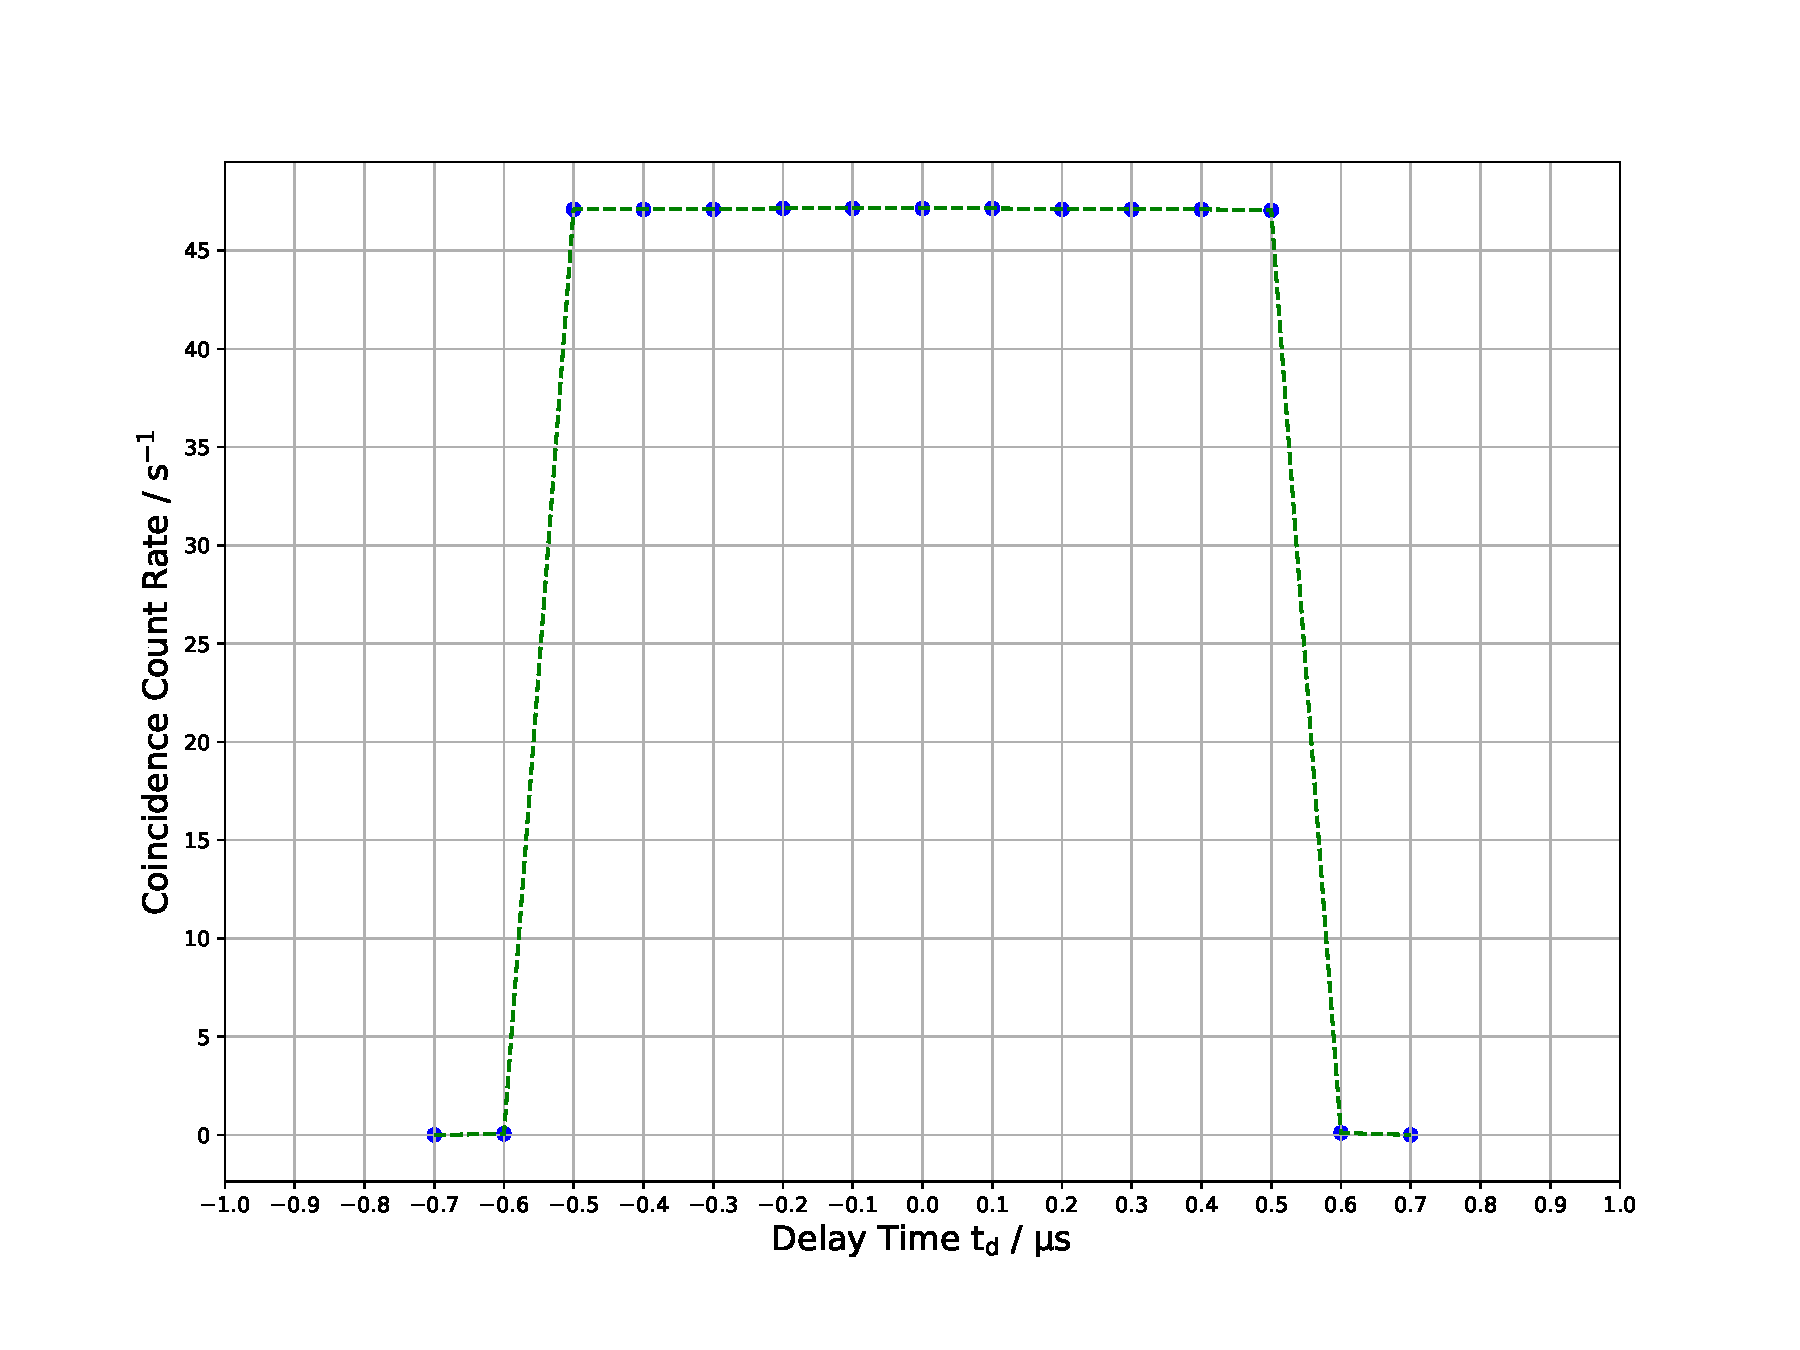
\includegraphics[height=12cm, width=16cm]{images/phyex1_fig.pdf}
 \caption{符合计数率画出的瞬时符合曲线}
 \label{fig:fig1}
\end{figure}\\\\
我们认为$0.6\mu s$附近矩形脉冲波形迅速降为0,这样可以得到矩形脉冲宽
\begin{equation}
    2\tau=1.20\mu s
\end{equation}
即电子学分辨时间为
\begin{equation}
    \tau=0.60\mu s
\end{equation}
\item 按实验装置图检查连接线路,将放射源$\mathrm \sideset{^{60}}{}Co$置于抽板上(注意:放射源的活性区面朝上).通过示波器观察经过线性放大器放大后的输出脉冲波形,调节线性放大器的放大倍数,使$\beta$道和$\gamma$道的脉冲幅度在+5~6V左右,调节单道的阈值为0.3~0.5V左右,工作模式为积分.重复步骤b,求出符合电路的物理分辨时间$\tau$.(注意:在符合分辨时间内,要求符合计数相对标准误差$\leq 1\%$,因此每个点的测量时间要求20秒).
输出脉冲波形如下图\ref{fig:fig2}. 
\begin{figure}[ht]
 \centering
 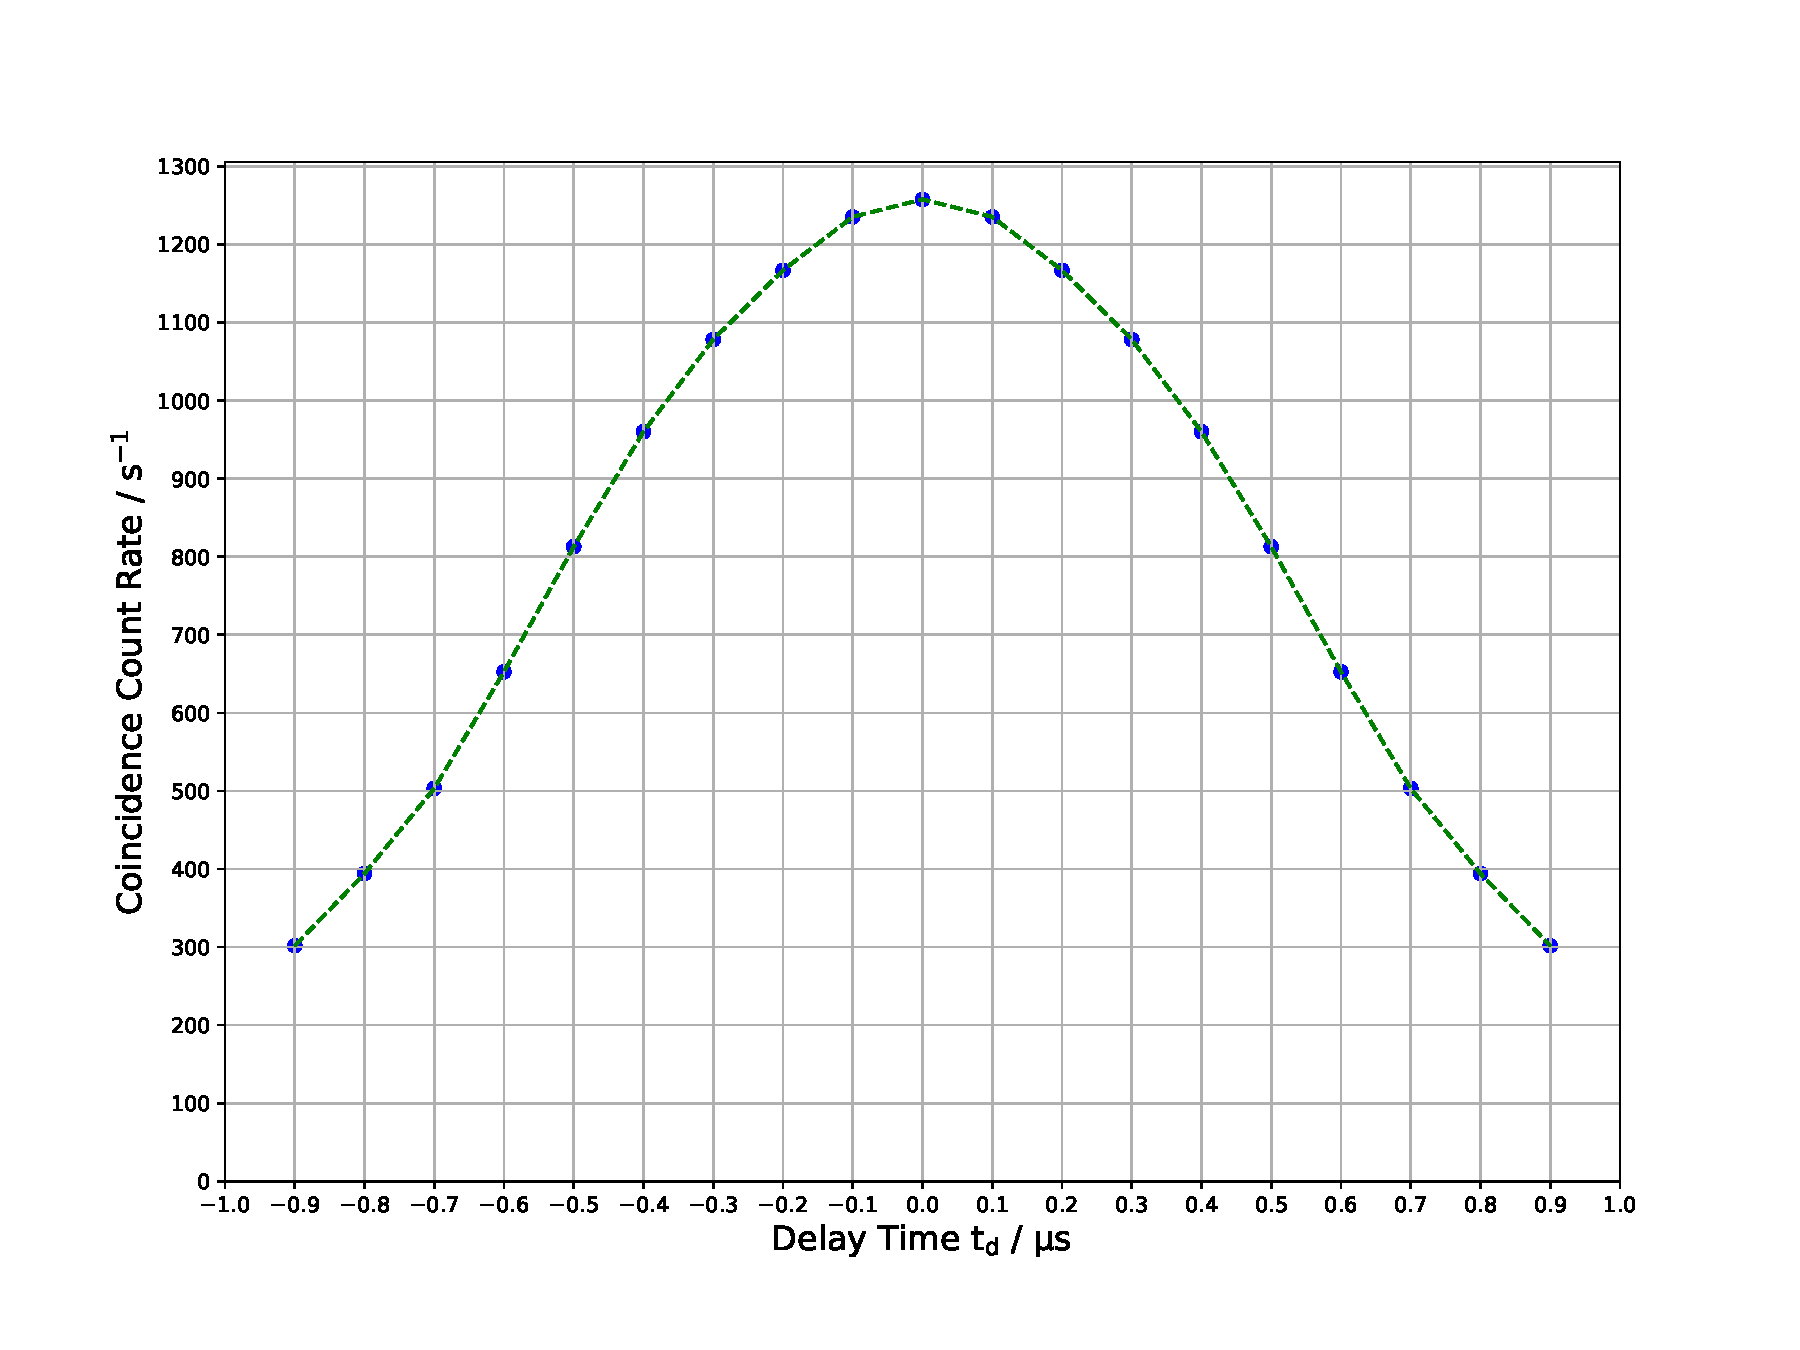
\includegraphics[height=12cm, width=16cm]{images/phyex2_fig.pdf}
 \caption{符合计数率表示的输出脉冲波形}
 \label{fig:fig2}
\end{figure}\\
我们对在$0.6\mu s$附近画出的脉冲波形做线性近似,这样可以得到半高宽
\begin{equation}
    2\tau^{\prime}=0.128\mu s
\end{equation}
即物理分辨时间为
\begin{equation}
    \tau^{\prime}=0.64\mu s
\end{equation}
\end{enumerate}

\begin{comment}
如果需要索引参考文献,请使用\cite{Erdos01}, 同时已经将参考文献的项目模版在文末写出。
\end{comment}

%------------------------------------------------------------
\newpage
\subsection{将两道的延迟时间调节到符合最佳位置,利用符合法测量放射源活度}\label{sub:ctl}
\begin{enumerate}[a)]
\item 在测量时间$T=20s$的条件下,测出有/无铝片时各个道/符合计数情况,(注意:每个量测量三遍,求平均值),如表~\ref{tab:table1}.
\begin{table}[htp]
\caption{$T=20s$内有/无铝片的三次各道/符合计数}\label{tab:table1}
\begin{center}\begin{tabular}{|c|c|c|c|c|c|}%p{6cm}|}
    \toprule
	\hline
	\multirow{2}{*}{\textbf{测量次数i}} & \multicolumn{3}{c|}{\textbf{无铝片}} & \multicolumn{2}{c|}{\textbf{有铝片}}\\
	\cline{2-6}
	& \textbf{$\beta$道计数$N_1$} & \textbf{$\gamma$道计数$N_2$} & \textbf{符合计数$N_c$} & \textbf{$\beta$道计数$N^{\prime}_1$} & \textbf{符合计数$N^{\prime}_c$}\\ \hline \hline
	$1$ & 161361 & 345052 & 24120 & 20503 & 2048\\ \hline
	$2$ & 160187 & 343662 & 23050 & 20780 & 2095\\ \hline
	$3$ & 159817 & 343463 & 23578 & 20505 & 2105\\ \hline
	平均 & 160455 & 344059 & 23582.67 & 20596 & 2082.67\\ \hline
	\bottomrule
	\end{tabular}
\end{center}
\end{table}\\
然后利用$m=\frac{N}{T}$,可以求出对应的计数率,如下表~\ref{tab:table2}.
\begin{table}[htp]
\caption{有/无铝片的各道/符合计数率}\label{tab:table2}
\begin{center}\begin{tabular}{|c|c|c|c|}%p{6cm}|}
    \toprule
	\hline
	\diagbox & \textbf{$\beta$道} & \textbf{$\gamma$道} & \textbf{符合}\\ \hline \hline
	\textbf{无铝片} & $m_1=8022.75/s$ & $m_2=17202.95/s$ & $m_c=1179.133/s$ \\ \hline
	\textbf{有铝片} & $m^{\prime}_1=1029.8/s$ & \diagbox & $m^{\prime}_c=104.133/s$ \\ \hline
	\bottomrule
	\end{tabular}
\end{center}
\end{table}\\
\item 然后取出$\mathrm \sideset{^{60}}{}Co$源,测量得到$\gamma$道本底计数率
\begin{equation}
    m^{bkg}_2=243.33/s
\end{equation}
\item 计算$\mathrm \sideset{^{60}}{}Co$源现时的绝对活度D及其误差:
这样现时的绝对活度D为
\begin{equation}
    D=\frac{(m_1-m^{\prime}_1)(m_2-m_2^{\prime})}{m_c-m^{\prime}_c-2\tau (m_1-m_1^{\prime})m_2}=1.186\times 10^5 Bq
\end{equation}
同时根据误差传递,算出$\sigma_D=0.02\times 10^5Bq$,则测量结果为
\begin{equation}
    D\pm \sigma_D=(1.19\pm0.02)\times 10^5 Bq
\end{equation}
已知待测放射源$\mathrm \sideset{^{60}}{}Co$编号CO1505号,在时刻$t_0=$2015年10月08日标定活度$D_0$为:$2.514\times 10^5 Bq$
测量时刻为$t_1=$2021年10月28日15:00, 可以算出经过时间为$t=t_1-t_0$.而半衰期$T=5.27$年,则计算出绝对活度的理论值为
\begin{equation}
    D_{th}=D_0 e^{-\lambda t}=D_0e^{-\frac{\ln{2}}{T}t}=1.134\times 10^5 Bq
\end{equation}
则相对误差为$\left|\frac{D-D_{th}}{D_{th}}\right|=4.6\%$
\end{enumerate}
%------------------------------------------------------------
%add more subsections for other block

%%%%%%%%%%%%%%%%%%%%%%%%%%%%%%%%%%%%%%%% Conclusion %%%%%%%%%%%%%%%%%%%%%%%%%%%%%%%%%%%%%%%%
\newpage
\section{结论}\label{conclusions}
由以上结果可见,测量得到的符合电路的物理分辨时间$\tau^\prime$接近电子学分辨时间$\tau$,都在$0.60\mu s$附近,符合我们的预期.

同时,测量得到的放射源$\mathrm \sideset{^{60}}{}Co$活度D与理论计算结果$D_{th}$误差在5\%以内,是我们可以接受的误差范围,进一步证明了符合测量的精确性和优越性.



%%%%%%%%%%%%%%%%%%%%%%%%%%%%%%%%%%%%%%%% Questions %%%%%%%%%%%%%%%%%%%%%%%%%%%%%%%%%%%%%%%%
\begin{comment}
\section{实验报告思考题}\label{questions}
\subsection{在$a=23.0mm$、$b=10.0mm$的矩形波导管中能不能传播$\lambda=2cm$、$3cm$和$5cm$的微波?各能传播哪些波型?}\label{sub:question1}
答:根据
\begin{equation}
    \lambda_c=\frac{2}{\sqrt{(m/a)^2+(n/b)^2}}
\end{equation}
我们可以算出可传播的最大波长为$\lambda_{max}=18.3mm$,显然不能传播$\lambda=2cm$、$3cm$和$5cm$的微波,可传输波长在$\lambda_{max}=18.3mm$以下,满足$\lambda_c=\frac{2}{\sqrt{(m/a)^2+(n/b)^2}}$的波长的波型\\

\end{comment}

%%%%%%%%%%%%%%%%%%%%%%%%%%%%%%%%%%%%%%%% Acknowledgements %%%%%%%%%%%%%%%%%%%%%%%%%%%%%%%%%%%%%%%%

\section{致谢}\label{acknowledgments}
感谢楼建玲老师在实验中的的悉心指导.

\begin{comment}
%%%%%%%%%%%%%%%%%%%%%%%%%%%%%%%%%%%%%%%% Appendix %%%%%%%%%%%%%%%%%%%%%%%%%%%%%%%%%%%%%%%%
\appendix
\section{代码}\label{sub:app.code}
请在附录\ref{sub:app.code}中添加代码。请使用如下Scala的语法高亮描述方法。
\begin{scala}
class TopIO extends Bundle() {
	val boot = Input(Bool()) 
// imem and dmem interface for Tests
	val test_im_wr		= Input(Bool())
	val test_im_rd 		= Input(Bool())
	val test_im_addr 	= Input(UInt(32.W))
	val test_im_in 		= Input(UInt(32.W))
	val test_im_out 	= Output(UInt(32.W))

	val test_dm_wr		= Input(Bool())
	val test_dm_rd 		= Input(Bool())
	val test_dm_addr 	= Input(UInt(32.W))
	val test_dm_in 		= Input(UInt(32.W))
	val test_dm_out 	= Output(UInt(32.W))

	val valid			= Output(Bool())
}
class Top extends Module() {
	val io 		= IO(new TopIO())//in chisel3, io must be wrapped in IO(...) 
	//...
	when (io.boot & io.test_im_wr){
		imm(io.test_im_addr) := io.test_im_in
		} .elsewhen (io.boot & io.test_dm_wr){
		// please finish it
		} //...
}
\end{scala}
\newpage

%%%%%%%%%%%%%%%%%%%%%%%%%%%%%%%%%%%%%%%% REFERENCE %%%%%%%%%%%%%%%%%%%%%%%%%%%%%%%%%%%%%%%%
\begin{thebibliography}{9}

\bibitem{Erdos01} P. Erd\H os, \emph{A selection of problems and
results in combinatorics}, Recent trends in combinatorics (Matrahaza,
1995), Cambridge Univ. Press, Cambridge, 2001, pp. 1--6.

\end{thebibliography}
\end{comment}
\end{document}

